	Praca nad niewidoczną dla użytkownika końcowego częścią generycznych modułów zaowocowała opracowaniem 3 niezależnych modułów. Działając po stronie serwera upraszczają pracę z takimi elementami, jak strony wyświetlające informacje o obiektach pochodzących z modelu danych, definiowanie nowych tabel i zbioru danych oraz ostatecznie tworzenie, zapisywanie i generowanie raportów biznesowych. 

\subsubsection{Strony obiektów domenowych oraz tabele}
	Komponenty istnieją w dwóch różnych wariantach. Wariant 1 służy do generowania stron dla obiektów biznesowych, zwanych dalej \textbf{info page}, natomiast zadaniem wariantu drugiego jest generowanie zarówno konfiguracji, jak i danych dla tabel. Oba rodzaje zostały zaprojektowane, aby zminimalizować ilość potrzebnych do przesłania danych. Powodem istnienia dwóch różnych klas jest różnica w konstrukcji strony HTML a tabeli. Dodatkowo w przypadku tabeli pewne charakterystyczne elementy, takie jak zmienne opisujące zachowanie kolumn czy też całej tabeli zostały wymuszone przez zastosowanie biblioteki \textbf{Dandelion Datatables} \ref{tech:dandelion}. 
	\begin{listing}[H]
		\inputminted[
			lineos=true,
			firstline=32,
			lastline=46,
			fontfamily=monospace,
			obeytabs=true,
			samepage=true,
			fontsize=\scriptsize
		]{java}{\SpringatomScrPath{/web/component/builders/ComponentBuilder.java}}
		% src file used
		\label{app:component_builder}
		\caption[\textbf{ComponentBuilder - korzeń hierarchii modułu komponentów}]{
			\textbf{ComponentBuilder} - korzeń hierarchii modułu komponentów, który
			wyznacz rolę tego rodzaju obiektów w systemie.					
		}
	\end{listing}
	
	Szczególnie ważne są tutaj następujące metody:
	\begin{itemize}
		\item \textbf{getDefinition()} - wywołanie następuje w momencie kiedy użytkownik otwiera
		stronę, w strukturze DOM, gdzie zapisana jest informacja o obiekcie biznesowym, pobrana z aktualnego adresu
		URL.
		\item \textbf{getData()} - jest to metoda zaprojektowana do wygenerowania
		asynchronicznej odpowiedzi \textbf{Ajax} na żądania pobrania gotowego widoku renderowanego komponentu.
	\end{itemize}

	Z uwagi na dwa oddzielne odnogi \textbf{ComponentBuilder}'ów w strukturze dziedziczenie oraz różnych wymogów, co do konstrukcji końcowego widoku prezentowanego użytkownikowi, istnieją także dwa kontrolery. Jeden z nich został zaprojektowany specjalnie dla \textbf{info page}. Rolą drugiego jest umożliwić generowanie tabel. 

	Poniższe listingi pokazują implementacje metod w warstwie kontrolerów odpowiednio wywołujących funkcje \textbf{getData()} oraz \textbf{getDefinition()}. 
	\begin{listing}[H]
		\inputminted[
			lineos=true,
			firstline=59,
			lastline=79,
			fontfamily=monospace,
			obeytabs=true, 
			samepage=true,
			fontsize=\scriptsize
		]{java}{\SpringatomScrPath{/webmvc/controllers/SVInfoPageController.java}}
		% src file used
		\caption[Obsługa żądania \textbf{ComponentBuilder\#{}getDefinition()}]{
			Obsługa żądania w kontrolerze, które wywołuje metodą \textbf{getDefinition()}
			dla strony domenowej
		}
		\label{app:infopage_ctrl_get_def}
	\end{listing}
	\begin{listing}[H]
		\inputminted[
			lineos=true,
			firstline=89,
			lastline=110,
			fontfamily=monospace,
			obeytabs=true, 
			samepage=true,
			fontsize=\scriptsize
		]{java}{\SpringatomScrPath{/webmvc/controllers/SVTableBuilderController.java}}
		% src file used
		\caption[Obsługa żądania \textbf{ComponentBuilder\#{}getData()}]{
			Obsługa żądania w kontrolerze, które wywołuje metodą \textbf{getData()}
			dla tabeli
		}
		\label{app:table_ctrl_get_data}
	\end{listing}

	Dla tabel istnieje możliwość zdefiniowania atrybutów do zaprezentowania
	użytkownikowi, które bezpośrednio nie istnieją w klasie odpowiadającej danemu obiektowi. Należy wtedy przeciążyć metodę
	\emph{handleDynamicColumn}, której zadaniem jest zwrócenie wartości dla danego, \textbf{dynamicznego} atrybutu.
	Poniższy kod pokazuje przykładową implementację:
	\begin{listing}[H]
		\inputminted[
			lineos=true,
			firstline=75,
			lastline=109,
			fontfamily=monospace,
			obeytabs=true, 
			samepage=true,
			fontsize=\scriptsize
		]{java}{\SpringatomScrPath{/web/rbuilder/table/ReportTableBuilder.java}}
		% src file used
		\caption[Uzyskania wartości dynamicznego atrybutu]{
			Uzyskania wartości dynamicznego atrybutu w momencie tworzenia
			odpowiedzi dla tabeli
		}
		\label{app:handleDynamicColumn}
	\end{listing}
	Zadaniem kodu na listingu \ref{app:handleDynamicColumn} jest zwrócenie akcji dla poszczególnych wierszy, które użytkownik będzie
	mógł wykonać na obiekcie odpowiadającym danemu rekordowi w tabeli. 

\pagebreak
\subsubsection{InfoPage - strony obiektów modelu danych}
	\textbf{InfoPage} jest komponentem prezentującym atrybuty danego obiektu domenowego w postaci strony internetowej. Dzięki wykorzystaniu informacji pobranych z meta modelu obiektów domenowych, utworzenie nowej strony sprowadza się do zaimplementowania rozszerzenia specjalnej klasy \emph{EntityInfoPageComponentBuilder}. Uzyskanie dostępu do danych i wkomponowanie ich do struktury drzewa nie wymaga w tym miejscu dalszej implementacji kodu o ile dany atrybut istnieje w klasie \textbf{Java}. W innym wypadku jest on atrybutem dynamicznym i należy zaimplementować kod, który zwróci jego wartość. Moduł jest wysoce generyczny i zautomatyzowany. Utworzenie strony dla nowego typu w modelu danych, które pojawiły by się w systemie, sprowadza się do utworzenia klasy, gdzie zdefiniowania zostanie struktura strony - panele oraz ich atrybuty. Warto w tym miejscu zaznaczyć, że tak zwany \textbf{panel systemowy} dodawany jest do każdej strony, jeśli powiązany z nią obiekt jest wersjonowany, tj. posiada historię zmian. 
	\begin{figure}[H]
		\centering
		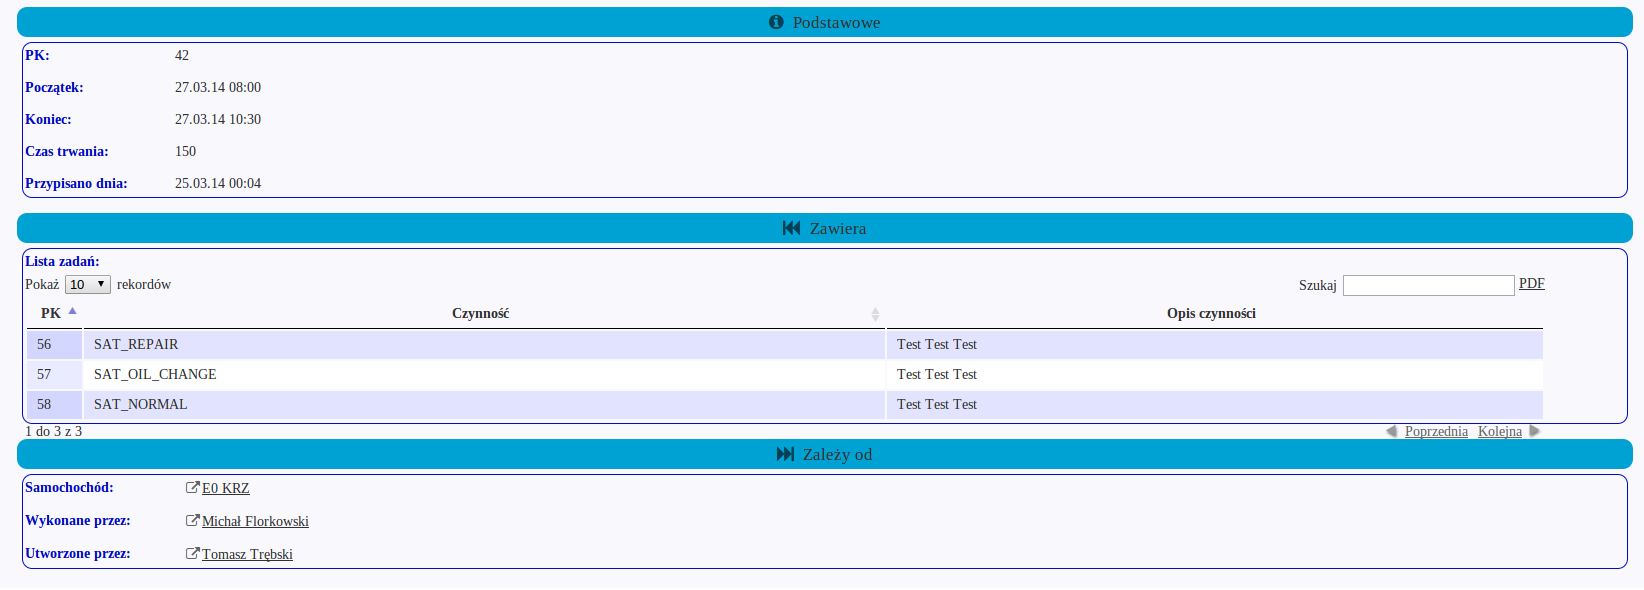
\includegraphics[width=1.0\textwidth]{images/infoPage}
		\caption[Strona domenowa dla spotkania]{
			Strona domenowa dla spotkania	
		}
		\label{app:infoPage}
	\end{figure}
	Na rysunku \ref{app:infoPage} pokazana została strona domenowa obiektu opisującego pojedyncza wizytę w warsztacie samochodowym. Zdefiniowane zostały 3 panele z atrybutami. Panel podstawowy oraz dwa opisujące relacje zachodzące między spotkaniem a innymi obiektami. Spotkanie posiada więc listę zadań oraz zostało przypisane do pewnego samochodu, zgłoszone i wykonane przez konkretnych mechaników. Listing kodu \ref{app:infoPageSrcCode} przedstawia kod Java odpowiedzialny za zbudowania struktury strony.
	\begin{listing}[H]
		\inputminted[
			lineos=true,
			firstline=37,
			lastline=76,
			fontfamily=monospace,
			obeytabs=true,
			samepage=true,
			fontsize=\scriptsize
		]{java}{\SpringatomScrPath{/webmvc/pages/builders/AppointmentInfoPageComponentBuilder.java}}
		\caption[Strona domenowa dla spotkania - kod źródłowy]{Strona domenowa dla spotkania - kod źródłowy}
		\label{app:infoPageSrcCode}
	\end{listing}

\pagebreak
\subsubsection{TableBuilder - definiowanie oraz dane dla tabel}
	Rzadko zdarza się żeby aplikacja nie wymagała korzystania z tabel do prezentowania danych. Są one szczególnie użyteczne zwłaszcza w momencie, kiedy ilość możliwych obiektów do jednorazowego wyświetlenia sięga co najmniej kilkudziesięciu elementów. W części praktycznej za obsługę tabel odpowiada biblioteka \textbf{Dandelion Datatables}. Renderowanie tabel oraz wsparcie dla funkcji takich jak sortowanie, filtrowanie. Niemniej ta biblioteka, podobnie jak wiele innych, nie posiada bezpośredniego wsparcia dla generowania struktur tabel oraz danych po stronie serwera, ze szczególnym naciskiem na definicję tabeli. Moduł \textbf{TableBuilder} rozwiązuje problemy takie jak:
	\begin{itemize}
		\item dynamiczna struktura tabel - to jakie kolumny będą widocznie zależne jest od dowolnych czynników,
		\item wsparcie dla sortowania po stronie serwera,
		\item wsparcie dla filtrowania po stronie serwera,
		\item zwracania danych tekstowych dla kolumn odpowiadających danym nie atomowym\footnote{Obiekt atomowy - pojedynczy, jeden. Obiekt nie atomowym to obiekt zwierający więcej niż jedną informację na raz},
		\item wsparcie dla dynamicznych kolumn, które nie odpowiadają żadnej z cech obiektów wyświetlanych w danej tabeli
	\end{itemize}
		
	\begin{listing}[H]
		\inputminted[
			lineos=true,
			firstline=35,
			lastline=76,
			fontfamily=monospace,
			obeytabs=true,
			samepage=true,
			fontsize=\scriptsize
		]{java}{\SpringatomScrPath{/webmvc/pages/builders/CarsTableBuilder.java}}
		% src file used
		\caption[Klasa definiująca strukturę tabeli wyświetlającej listę samochodów]{
			\emph{CarsTableBuilder} - klasa definiująca strukturę tabeli wyświetlającej listę samochodów	
		}
		\label{app:cars_table_src_code}
	\end{listing}
	
\subsubsection{RBuilder - raporty biznesowe}
	\textbf{RBuilder} jest praktyczną realizacją, będącej na wczesnym etapie rozwoju, koncepcji zaprojektowania generycznego
	silnika raportowania dla aplikacji internetowej. Głównymi założeniami tego komponentu są:
	\begin{itemize}
		\item możliwość generowania raportów przez użytkowników systemu,
		\item możliwość zapisywania raportów do bazy danych, celem późniejszego ich użycia,
		\item możliwość edycji istniejących raportów,
		\item możliwość usuwania istniejących raportów,
		\item wsparcie dla zabezpieczenie akcji możliwych do wykonania na raportach,
		\item eksport raportów do formatów:
		\begin{itemize}	\label{app:rbuilder_representations}
			\item PDF
			\item XLS
			\item HTML
			\item CSV
		\end{itemize}
	\end{itemize}		
	Jest to obecnie najbardziej skomplikowany komponent aplikacji, którego złożoność jeszcze wzrośnie, z uwagi
	na założenie, że raporty mogą być definiowane przez użytkowników. 
	
	Definiowanie raportu przebiega według następujących kroków:
	\begin{enumerate}
		\item Użytkownik wybiera z listy tabele dla których chce wygenerować raport,
		\item Dla zaznaczonych tabel użytkownik wybiera kolumny oraz format, w jakim zostaną wyświetlone,
		\item Użytkownik podaje informacje takie jak:
		\begin{itemize}
			\item nazwa
			\item opis
		\end{itemize}
		\item Sterowanie jest przekazywane do serwisu odpowiedzialnego za:
		\begin{itemize}
			\item zdecydowanie o rodzaju raportu: dla jednej tabeli, dla wielu tabel,
			\item utworzenie obiektu domenowego raportu zawierającego informację takie jak tytuł,
			\item utworzenie, kompilacja i zapisanie zserializowanego obiektu klasy \textbf{DynamicReport} do systemu plików,
			\item zwrócenie sterowania do \textbf{Spring Web Flow}
		\end{itemize}
		\item Generowanie raportu jest dostępne z tabeli zawierającej listę wszystkich raportów
	\end{enumerate}
	
	Report należy w tym miejscu rozumieć jako obiekt domenowy, który służy do późniejszego zapisanie
	wymaganych informacji do bazy danych oraz jako obiekt \textbf{Dynamic Jasper Report}. Celem dla którego
	tworzony jest ten obiekt leży w wykorzystanej bibliotece \textbf{DynamicJasper}. 
	Aby raport mógł być zaprezentowany użytkowniki, musi on zostać w pierwszej kolejności
	skompilowany do pliku \textit{*.jasper}. Załadowanie, a dokładniej odczytanie tego obiektu z zserializowanego
	pliku, zapisanego w systemie plików, jest wymogiem koniecznym i dostatecznym, aby sterowanie procesem
	tworzenie jednej z reprezentacji przekazać do szkieletu aplikacji \textbf{Spring}. Niemniej nie jest to jedyny
	wymóg. W specjalnej mapie, pod jasno określonymi kluczami, musi znaleźć się źródło danych dla raportu spójne z jego budową.
	Powyższe powody generują wiele niedogodności takich jak konieczność przechowywania dodatkowych plików na serwerze oraz
	trudności w uogólnieniu niektórych aspektów projektowania nowego raportu.
	
	Model danych przeznaczony dla \textbf{RBuilder} jest pewnym rozszerzeniem informacji o 
	danych biznesowych (domain object). Zawarte w nim informacje pozwalają na stwierdzenie następujących
	właściwości obiektów domenowych:
	\begin{itemize}
		\item nazwa tabeli,
		\item lokalizowana nazwa tabeli,
		\item atrybuty,
		\item powiązania z innymi modelami.
	\end{itemize}
	
	Późniejsze instancje obiektów zaprezentowanych na diagramie UML są wykorzystywane do przechowywania
	informacji niezbędnych do prawidłowego utworzenia konfiguracji raportu \textbf{ReportConfiguration}.
	
	\begin{figure}[H]
		\centering
		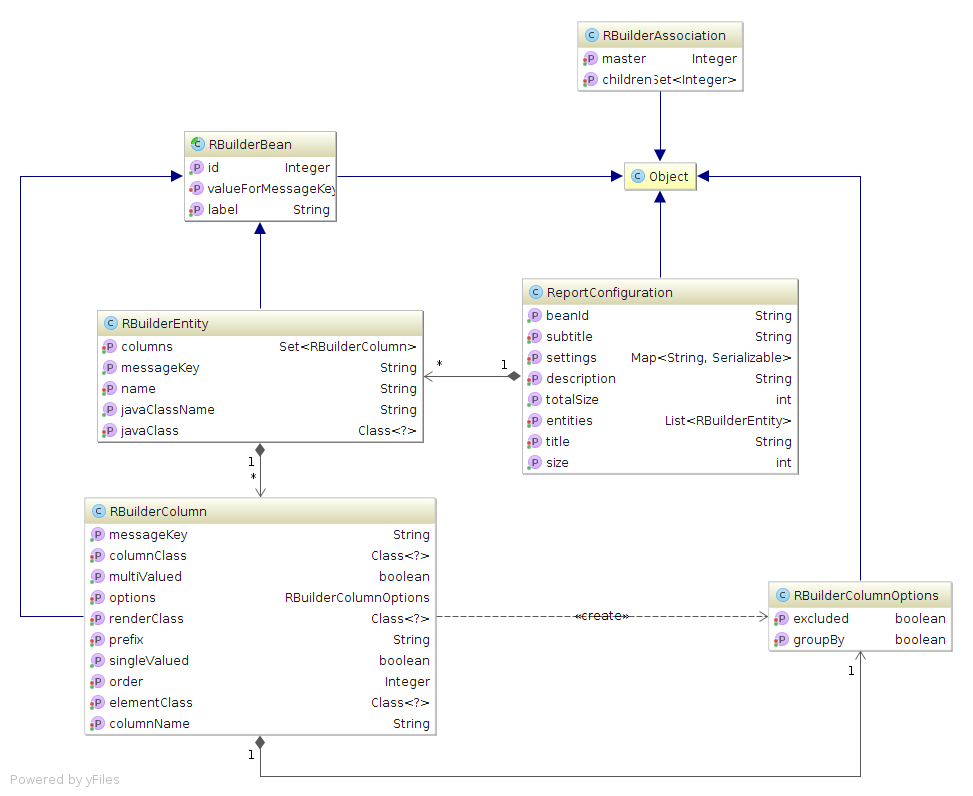
\includegraphics[width=1.0\textwidth]{images/rbuilder_dataModel}
		\caption[Diagram UML modelu danych \textbf{RBuilder}]{
			Diagram UML modelu danych \textbf{RBuilder}
		}
		\label{app:rbuilder_data_Model}
	\end{figure}	
	
	Serwisy \textbf{RBuilder}'a dostarczają metod, dzięki którym możliwe jest przygotowanie gotowego raportu
	w wybranej przez użytkownika reprezentacji i wsparcia dla przewodnika tworzenia nowego raportu. Dostarczone usługi to:
	\begin{itemize}
		\item ustalenie możliwych formatów danego atrybuty, a tym samym kolumny w raporcie,
		\item tworzenie obiektu domenowego w zależności od konfiguracji raportu,
		\item generowanie raportu,
		\item zapis i odczyt informacji o raporcie z bazy danych oraz systemu plików.
	\end{itemize}
	Funkcjonalność tej grupy klas dla komponentu \textbf{RBuilder} można podzielić na następujące bloki:
	\begin{center}
		\begin{longtable}{| p{2.5cm} | p{13cm} |}
			\caption[Bloki funkcjonalne modelu serwisów \textbf{RBuilder}]{
				Bloki funkcjonalne modelu serwisów \textbf{RBuilder}			
			}
			\label{app:rbuilder_services_functionality_table}
			\tabularnewline	
			
			\hline
				\multicolumn{1}{|c|}{\textbf{Grupa}} &
				\multicolumn{1}{|c|}{\textbf{Funkcjonalność}} \tabularnewline
			\hline
			\endfirsthead
			
			\multicolumn{2}{c}
			{{\bfseries \tablename\ \thetable{} -- kontynuacja...}} \tabularnewline
			\hline
				\multicolumn{1}{|c|}{\textbf{Grupa}} &
				\multicolumn{1}{|c|}{\textbf{Funkcjonalność}} \tabularnewline
			\hline
			\endhead
				
			\hline
				\multicolumn{2}{|r|}{{Następna strona...}} \tabularnewline \hline
			\endfoot
			\hline
			\endlastfoot	
			
			\emph{Operation Management} 									& 
			Grupa \textbf{Operation Management} odpowiedzialna jest za tworzenie obiektu \textbf{SReport} w zależności
			od ilości tabel wybranych dla konkretnego raportu. Lista klas:
			\begin{itemize}
				\item RBuilderOperation
				\item RBuilderCreateOperation
				\item SingleEntityRBuilderCreateOperation
				\item MultipleEntitiesRBuilderCreateOperation
			\end{itemize}					
			\hline
			\emph{Data Management}											&
			Klasy z grupy \textbf{Data Management} zostały zaprojektowane do pobierania danych takich jak:
			\begin{itemize}
				\item informacje o typach obiektów domenowych, które można uwzględnić w raportach. Takie klasy adnotowane są 
				przez \emph{\@{}ReportableEntity}, a ich lista udostępniana jest poprzez interfejs \emph{ReportableEntityResolver},
				\item listę kolumn wraz z ich cechami takimi jak nazwa, typ danych rzechowywanych w odpowiadającej jej polu w klasie, odpowiednie typu na które można rzutować dany typ. Informacje tego typu udostępniane są poprzez interfejs \emph{ReportableBeanResolver},
				\item listę powiązań między modelami w uproszczonej formie na potrzeby wybierania tabel podczas projektowania raportu. 
				Na obecną chwile możliwe jest utworzenie jedynie nieprzechodnich powiązań opisanych na bazowym poziomie przez relacje
				klucz główny - obcy. Dane tego typu udostępnione są przez interfejs \emph{ReportableAssociationResolver}. 
			\end{itemize}
			\hline
			\emph{Dynamic Jasper Operation}								&
			\emph{JasperBuilderService} jest jedyną klasą tej grupy, dostarczającą możliwości utworzenia skompilowanego
			raportu typu \textbf{JasperReport}, który potem jest serializowany do systemu plików. Niemniej jej głównym zadaniem
			jest wkomponowanie w obiekty wyżej wymienionego typu takich danych jak:
			\begin{itemize}
				\item tytuł,
				\item podtytuł,
				\item opis,
				\item język,
				\item szerokość odpowiednich sekcji jak nagłówek, stopka itp.,
				\item lista kolumn,
				\item lista kolumn według których dane mają być grupowane.
			\end{itemize}
			\hline
			\emph{View helper}												&
			\emph{ReportBuilderService} jest interfejsem serwisu, którego celem istnienia jest przekazanie sterowania do modułu
			\textbf{Operation Management}, celem utworzenia instancji obiektu domenowego \textbf{SReport} oraz wsparcie
			dla operacji renderowania raportu w konkretnej reprezentacji. Kiedy pierwsza z funkcji jest trywialna w kontekście złożoności, służąc
			jedynie separacji zadań i zmniejszeniu kohezji klas, druga z wymienionych metod jest dużo bardziej złożona.
			Jej celem jest pobranie danych wymaganych przez moduł \textbf{Spring}, używanych później do zrenderowania raportu 
			w wybranej reprezentacji, na przykład PDF. Operacje przez nią wykonywane to:
			\begin{itemize}
				\item pobranie obiektu domenowego z bazy danych dla danego numeru raportu, 
				\item deserializacja skompilowanego pliku \textit{*.jasper} z systemu plików,
				\item utworzenie źródła danych na podstawie informacji takich jak lista kolumn, ich typ, wybranych typ reprezentacji danych w kolumnie
			\end{itemize}
			\hline
		\end{longtable}
	\end{center}
				 
	Na część obsługującą widok komponentu \textbf{RBuilder} składają się:
	\begin{itemize}
		\item tabela z istniejącymi raportami \label{app:rbuilder_table},
		\item przewodnik tworzenia nowego raportu \label{app:rbuilder_wizard},
		\item specjalnie skonfigurowany \textbf{ViewResolver} \footnote{\href{http://docs.spring.io/spring/docs/current/javadoc-api/org/springframework/web/servlet/ViewResolver.html}{ViewResolver} - interfejs, które implementują specjalne klasy zadaniem których jest ładowanie widoków poprzez odwołanie m.in. do plików JSP, logicznych nazw widoków itp.}.
	\end{itemize}

	Tabela (\ref{app:rbuilder_table}) jest obiektem należącym do warstwy widoku, który został utworzony z użyciem komponentu
	tabeli. Zawiera ona dodatkowo akcje, umożliwiające operacje na raportach. 
	% dodać IMG			
	
	Przewodnik (\ref{app:rbuilder_wizard}) został zaprojektowany na podstawie \textbf{Spring Web Flow}. Dzięki 
	temu zbiór formularzy, na których definiuje się poszczególne elementy składowe gotowego obiektu \textbf{ReportConfiguration}
	(stanowiącego bazę do generowania wybranej reprezentacji \ref{app:rbuilder_representations} reportu), jest logicznie
	połączony. Dodatkową korzyścią jest uzyskanie bezproblemowego wsparcia dla przetwarzania danych wejściowych 
	po stronie serwera bez konieczności pisania własnej logiki do zarządzania komunikacją Ajax oraz możliwość przekazywania
	danych między kolejnymi krokami. 
	\begin{figure}[H]
		\centering
		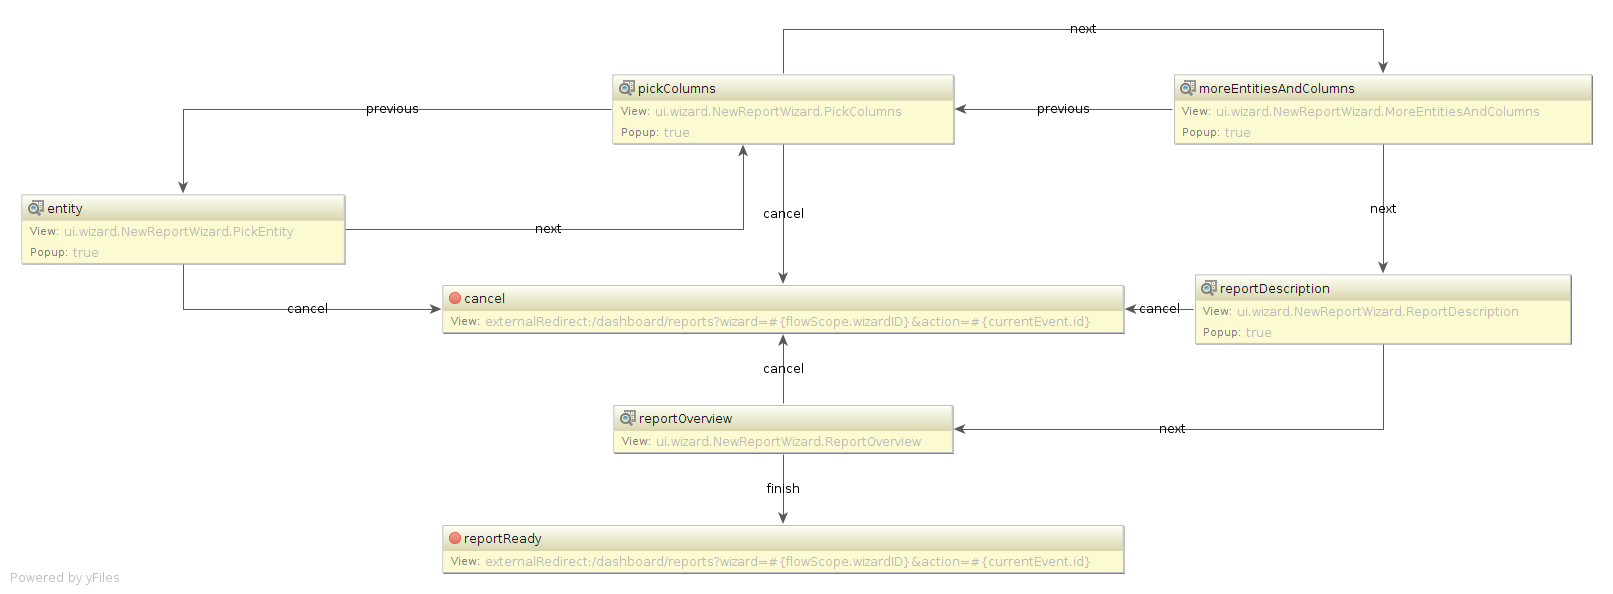
\includegraphics[width=1.0\textwidth]{images/rbuilder_flow}
		\caption[Logiczne połączenie kroków w przewodniku dla \textbf{RBuilder}]{
			Logiczne połączenie kroków w przewodniku dla \textbf{RBuilder}
		}
		\label{app:rbuilder_diagram_of_flow}
	\end{figure}
	Każdy z kroków przewodnika wspiera odpowiednia klasa Java, będąca specjalizowanym rozszerzeniem \href{http://docs.spring.io/spring-webflow/docs/2.4.0.M1/api/org/springframework/webflow/action/FormAction.html}{FormAction}, zarządzającą ustawieniem danych wejściowych
	dla formularza, walidacji i konwerterów. Ostatecznie jest to rzecz szczególnie ważna, ponieważ praktycznie wszystkie formularze
	zostały napisana aby wspierać wprowadzanie danych dla więcej niż jednego obiektu. Z uwagi na brak natywnego wsparcia ze strony
	szkieletu aplikacji \textbf{Spring} należało napisać odpowiednie metody, tworzące z prostych łańcuchów
	znakowych poprawne obiekty opisujące nowy raport. 
	\begin{listing}[H]
		\inputminted[
			lineos=true,
			firstline=151,
			lastline=169,
			fontfamily=monospace,
			obeytabs=true, 
			samepage=false,
			fontsize=\scriptsize
		]{java}{\SpringatomScrPath{/web/flows/wizards/wizard/rbuilder/PickEntityFormAction.java}}
		% src file used
		\caption[Bazowy konwerter dla operacji \textbf{PickEntityFormAction}]{
			Bazowy konwerter dla operacji \textbf{PickEntityFormAction} który tworzy z łańcuchów
			znakowych obiekty \textbf{RBuilderEntity}
		}
		\label{app:rbuilder_converter_of_data}
	\end{listing}